{\let\cleardoublepage\clearpage\chapter{Missa Catechumenorum}}

\directio{genuflectens}

\textit{%
    Sacerdos paratus cum ingreditur ad altare, facta illi debita reverentia,
    signat se signo crucis a fronte ad pectus, et, nisi peculiari rubrica aliter
    statuatur, clara voce dicit:
}

\initialis[3]{I}n nomine Patri, \cross{} et Filii, et Spiritus Sancti.  Amen.

\hspace{0.5em}\textit{Deinde, iunctis manibus ante pectus, incipit antiphonam:}

\versiculum{Introibo ad altare Dei.}

\textit{Ministri respondent:}

\responsorium{Ad Deum qui laetificat iuventutem meam.}

\textit{Postea alternatim cum ministris dicit sequentem:}

\biblia{Ps. 42, 1-5}

\initialis{I}udica me, Deus, et discerne causam meam de gente non sancta: ab
homine iniquo, et doloso erue me.

\minister{%
    Quia tu es, Deus, fortitudo mea: quare me repulisti, et quare tristis
    incedo, dum affligit me inimicus?
}
\alternatim{
    \par\sacerdos{%
        Emitte lucem tuam, et veritatem tuam: ipsa me deduxerunt, et adduxerunt
        in montem sanctum tuum, et in tabernacula tua.
    }
    \par\minister{%
        Et introibo ad altare Dei: ad Deum qui laetificat iuventutem meam.
    }
    \par\sacerdos{%
        Confitebor tibi in cithara, Deus, Deus meus: quare tristis es, anima
        mea, et quare conturbas me?
    }
    \par\minister{%
        Spera in Deo, quoniam adhuc confitebor illi: salutare vultus mei, et
        Deus meus.
    }
    \par\sacerdos{Gloria Patri, et Filio, et Spiritui Sancto.}
    \par\minister{%
        Sicut erat in principio, et nunc, et semper: et in saecula saeculorum.
        Amen.
    }
}

\textit{Sacerdos repetit antiphonam:}

\versiculum{Introibo ad altare Dei.}
\alternatim{\par\responsorium{Ad Deum qui laetificat iuventutem mean.}}

\textit{Signat se, dicens:}

\versiculum{Adiutorium nostrum \cross{} in nomine Domini.}
\alternatim{\par\responsorium{Qui fecit caelum et terram.}}

\textit{Deinde, iunctis manibus, profunde inclinatus facit confessionem.}

\pagebreak

\divisio

\textit{In Missis defunctorum, et in Missis de Tempore a dominica I Passionis
usque ad feriam V in Cena Domini inclusive, omittitur psalmus} Iudica me, Deus,
\textit{cum} Gloria Patri, \textit{et repetitione antiphonae, sed dicto} In
nomine Patris, Introibo, \textit{et} Adiutorium, \textit{fit confessio, ut
sequitur}:

\divisio

\section{Confiteor}

\initialis{C}onfiteor Deo omnipotenti, beatae Mariae semper Virgini, beato
Michaeli Archangelo, beato Ioanni Baptistae, sanctis Apostolis Petro et Paulo,
omnibus Sanctis, et vobis, fratres: quia peccavi nimis cogitatione, verbo et
opere: (\textit{percutit sibi pectus ter, dicens:}) mea culpa, mea culpa, mea
maxima culpa.  Ideo precor beatam Mariam semper Virginem, beatum Michaelem
Archangelum, beatum Ioannem Baptistam, sanctos Apostolos Petrum et Paulum, omnes
Sanctos, et vos, fratres, orare pro me ad Dominum Deum nostrum.

\textit{Ministri respondent:}

\initialis{M}isereatur tui omnipotens Deus, et, dimissis peccatis tuis, perducat
te ad vitam aeternam.

\textit{Sacerdos dicit:}

\versiculum{Amen.}

\textit{et erigit se.  Deinde ministri repetunt confessionem: et ubi a sacerdote
dicebatur} vobis, fratres, \textit{et} vos, fratres, \textit{a ministris
dicitur} tibi, pater, \textit{et} te, pater.  \textit{Postea sacerdos, iunctis
manibus, facit absolutionem, dicens:}

\initialis{M}iseratur vestri omnipotens Deus, et, dimissis peccatis vestris,
perducat vos ad vitam aeternam.

\responsorium{Amen.}

\textit{Signat se signo crucis, dicens:}

\initialis{I}ndulgentiam, \cross{} absolutionem et remissionem peccatorum
nostrorum tribuat nobis omnipotens et misericors Dominus.

\responsorium{Amen.}
\alternatim{
    \par\textit{Et inclinatus prosequitur:}
    \par\versiculum{Deus, tu conversus vivificabis nos.}
    \par\responsorium{Et plebs tua laetabitur in te.}
    \par\versiculum{Ostende nobis, Domine, misericordiam tuam.}
    \par\responsorium{Et salutare tuum da nobis.}
    \par\versiculum{Domine, exaudi orationem meam.}
    \par\responsorium{Et clamor meus ad te veniat.}
    \par\versiculum{Dominus vobiscum.}
    \par\responsorium{Et cum spiritu tuo.}
}

\textit{Et, extendens ac iungens manus, clara voce dicit:}

\versiculum{Oremus.}

\directio{stans}

\textit{et, ascendens ad altare, dicit secreto:}

\initialis{A}ufer a nobis, quaesumus, Domine, iniquitates nostras: ut ad Sancta
sanctorum puris mereamur mentibus introire.  Per Christum Dominum nostrum.
Amen.

\textit{Deinde, manibus iunctis super altare, inclinatus dicit:}

\initialis{O}ramus te, Domine, per merita Sanctorum tuorum, (\textit{osculatur
altare in medio}) quorum reliquiae hic sunt, et omnium Sanctorum: ut indulgere
digneris omnia peccata mea.  Amen.

\textit{%
    In Missa solemni, quae non sit defunctorum, celebrans, antequam incipiat
    antiphonam ad Introitum, benedicit incensum, dicens:
}

\sacerdos{Ab illo bene\cross{}dicaris, in cuius honore cremaberis.  Amen.}

\textit{%
    Et, accepto thuribulo a diacono, incensat altare, nihil dicens.  Postea
    diaconus, recepto thuribulo a celebrante, incensat illum tantum.
}

\section{Introitus}

\proprius{Introitus}

\textit{%
    Deinde celebrans, signans se signo crucis, incipit antiphonam ad Introitum
    qua finita, iunctis manibus, alternatim cum ministris dicit:
}

\section{Kyrie Eleison}

\begin{wrapfigure}{r}{0.6\textwidth}
    \centering
    \vspace{-0.5\baselineskip}
    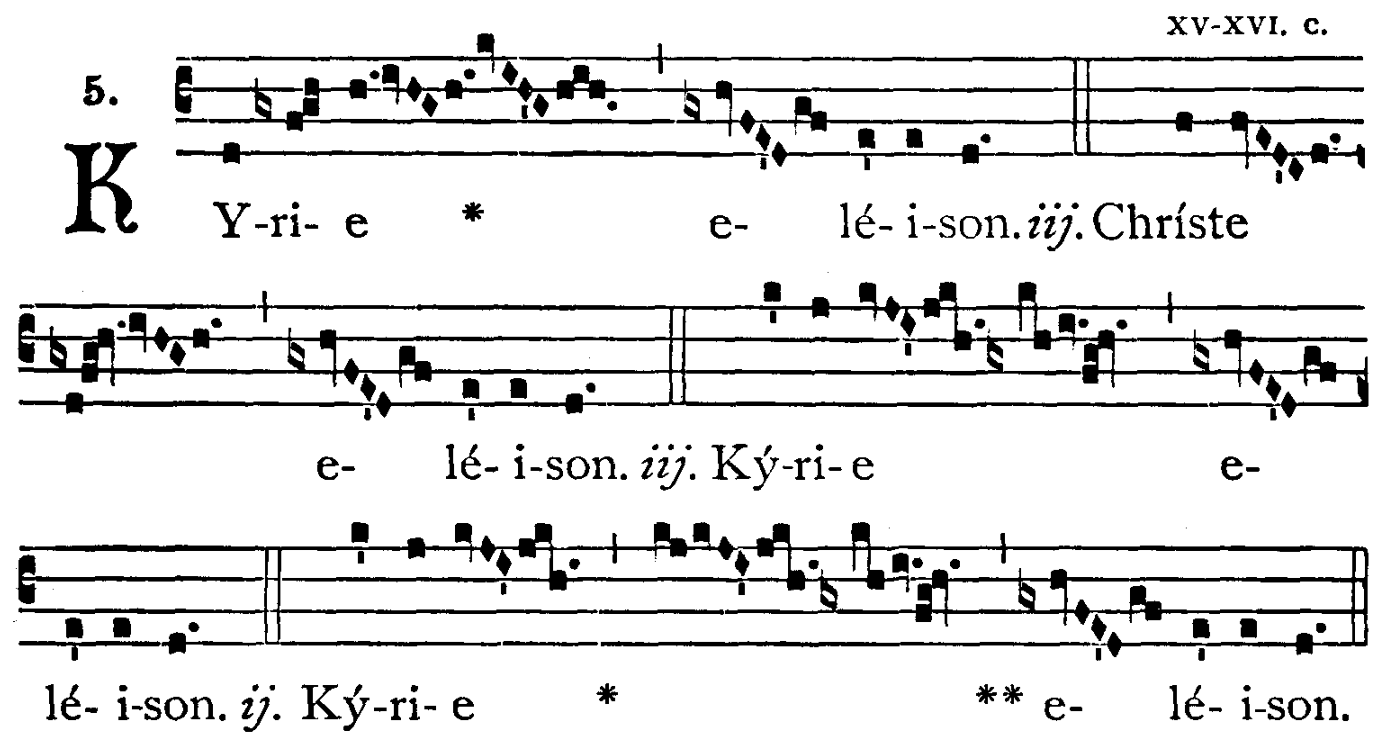
\includegraphics
        [scale=0.3, clip, viewport=2cm 17.5cm 22.5cm 25cm]
        {img/kyrie.png}
\end{wrapfigure}

\initialis{K}yrie, eleison. Kyrie, eleison. \\ Kyrie, eleison. \\
Christe, eleison.  Christe eleison. \\ Christe eleison. \\
Kyrie eleison.  Kyrie eleison. \\ Kyrie eleison.

\section{Gloria in Excelsis}

\begin{wrapfigure}{r}{0.5\textwidth}
    \centering
    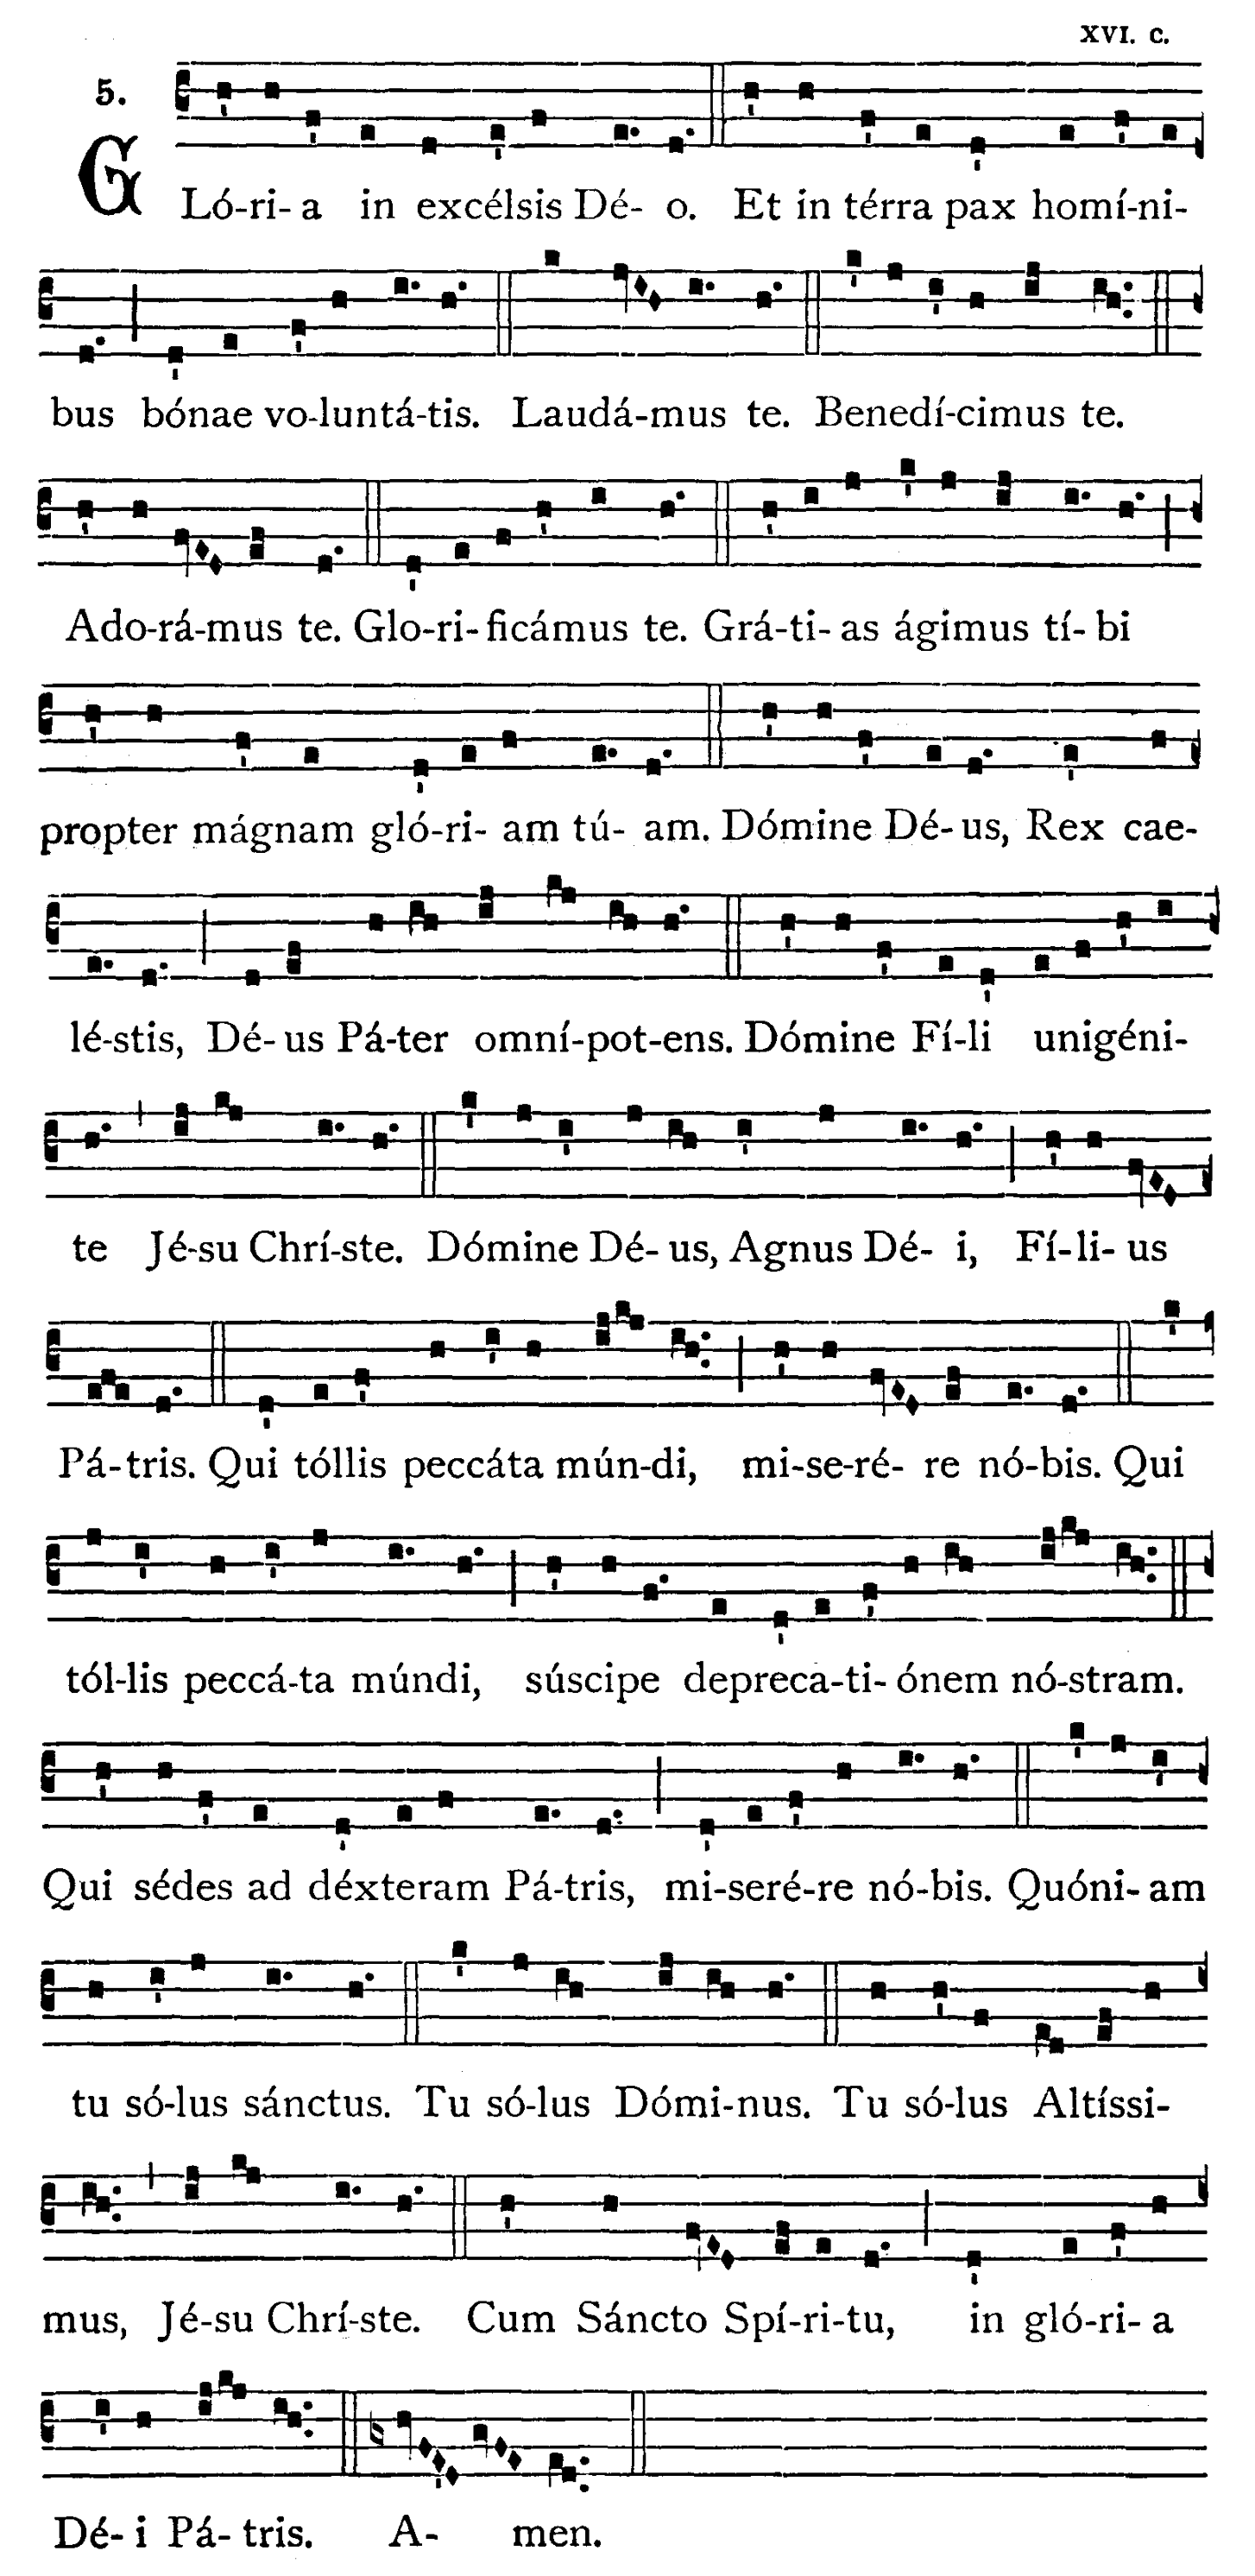
\includegraphics
        [scale=0.3, clip, viewport=3cm 96cm 29cm 103cm]
        {img/gloria.png}
\end{wrapfigure}

\begin{figure}[p]
    \centering
    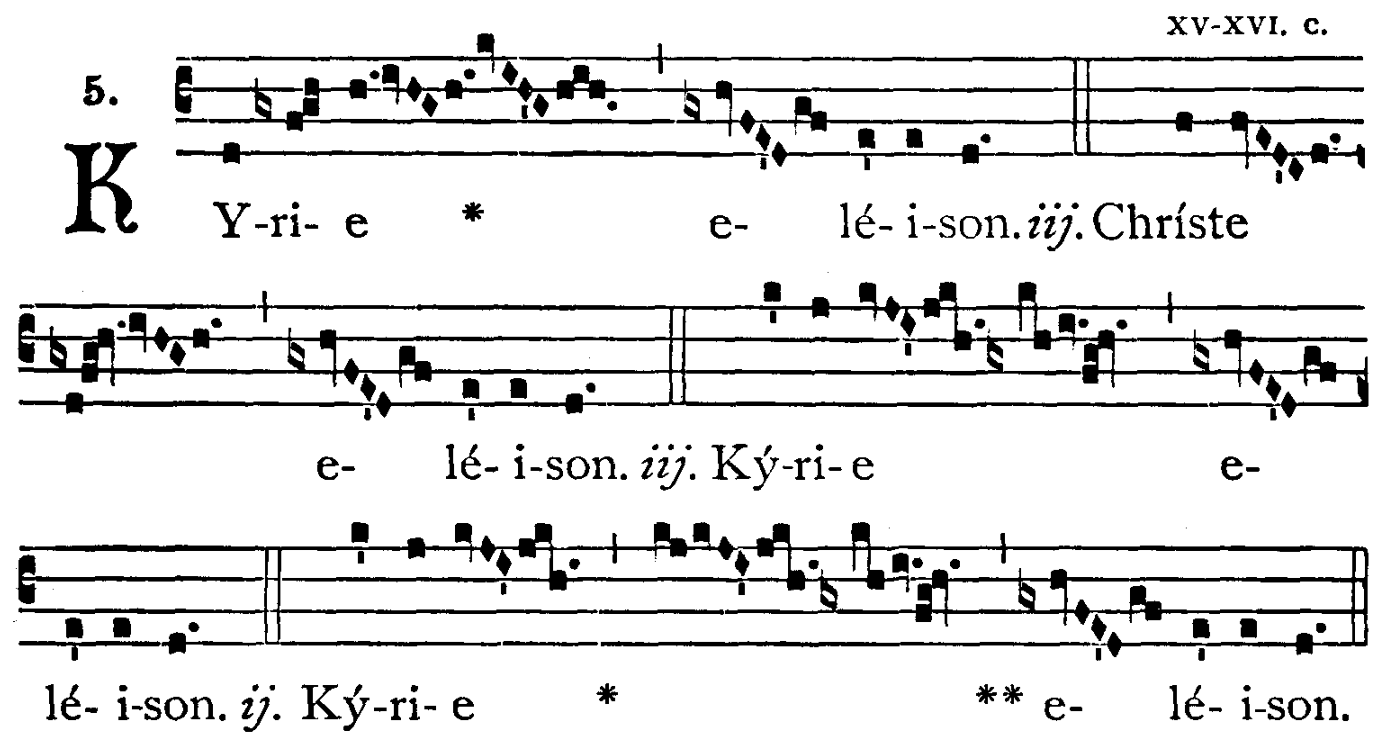
\includegraphics[scale=0.3]{img/kyrie.png}
    \\[2\baselineskip]
    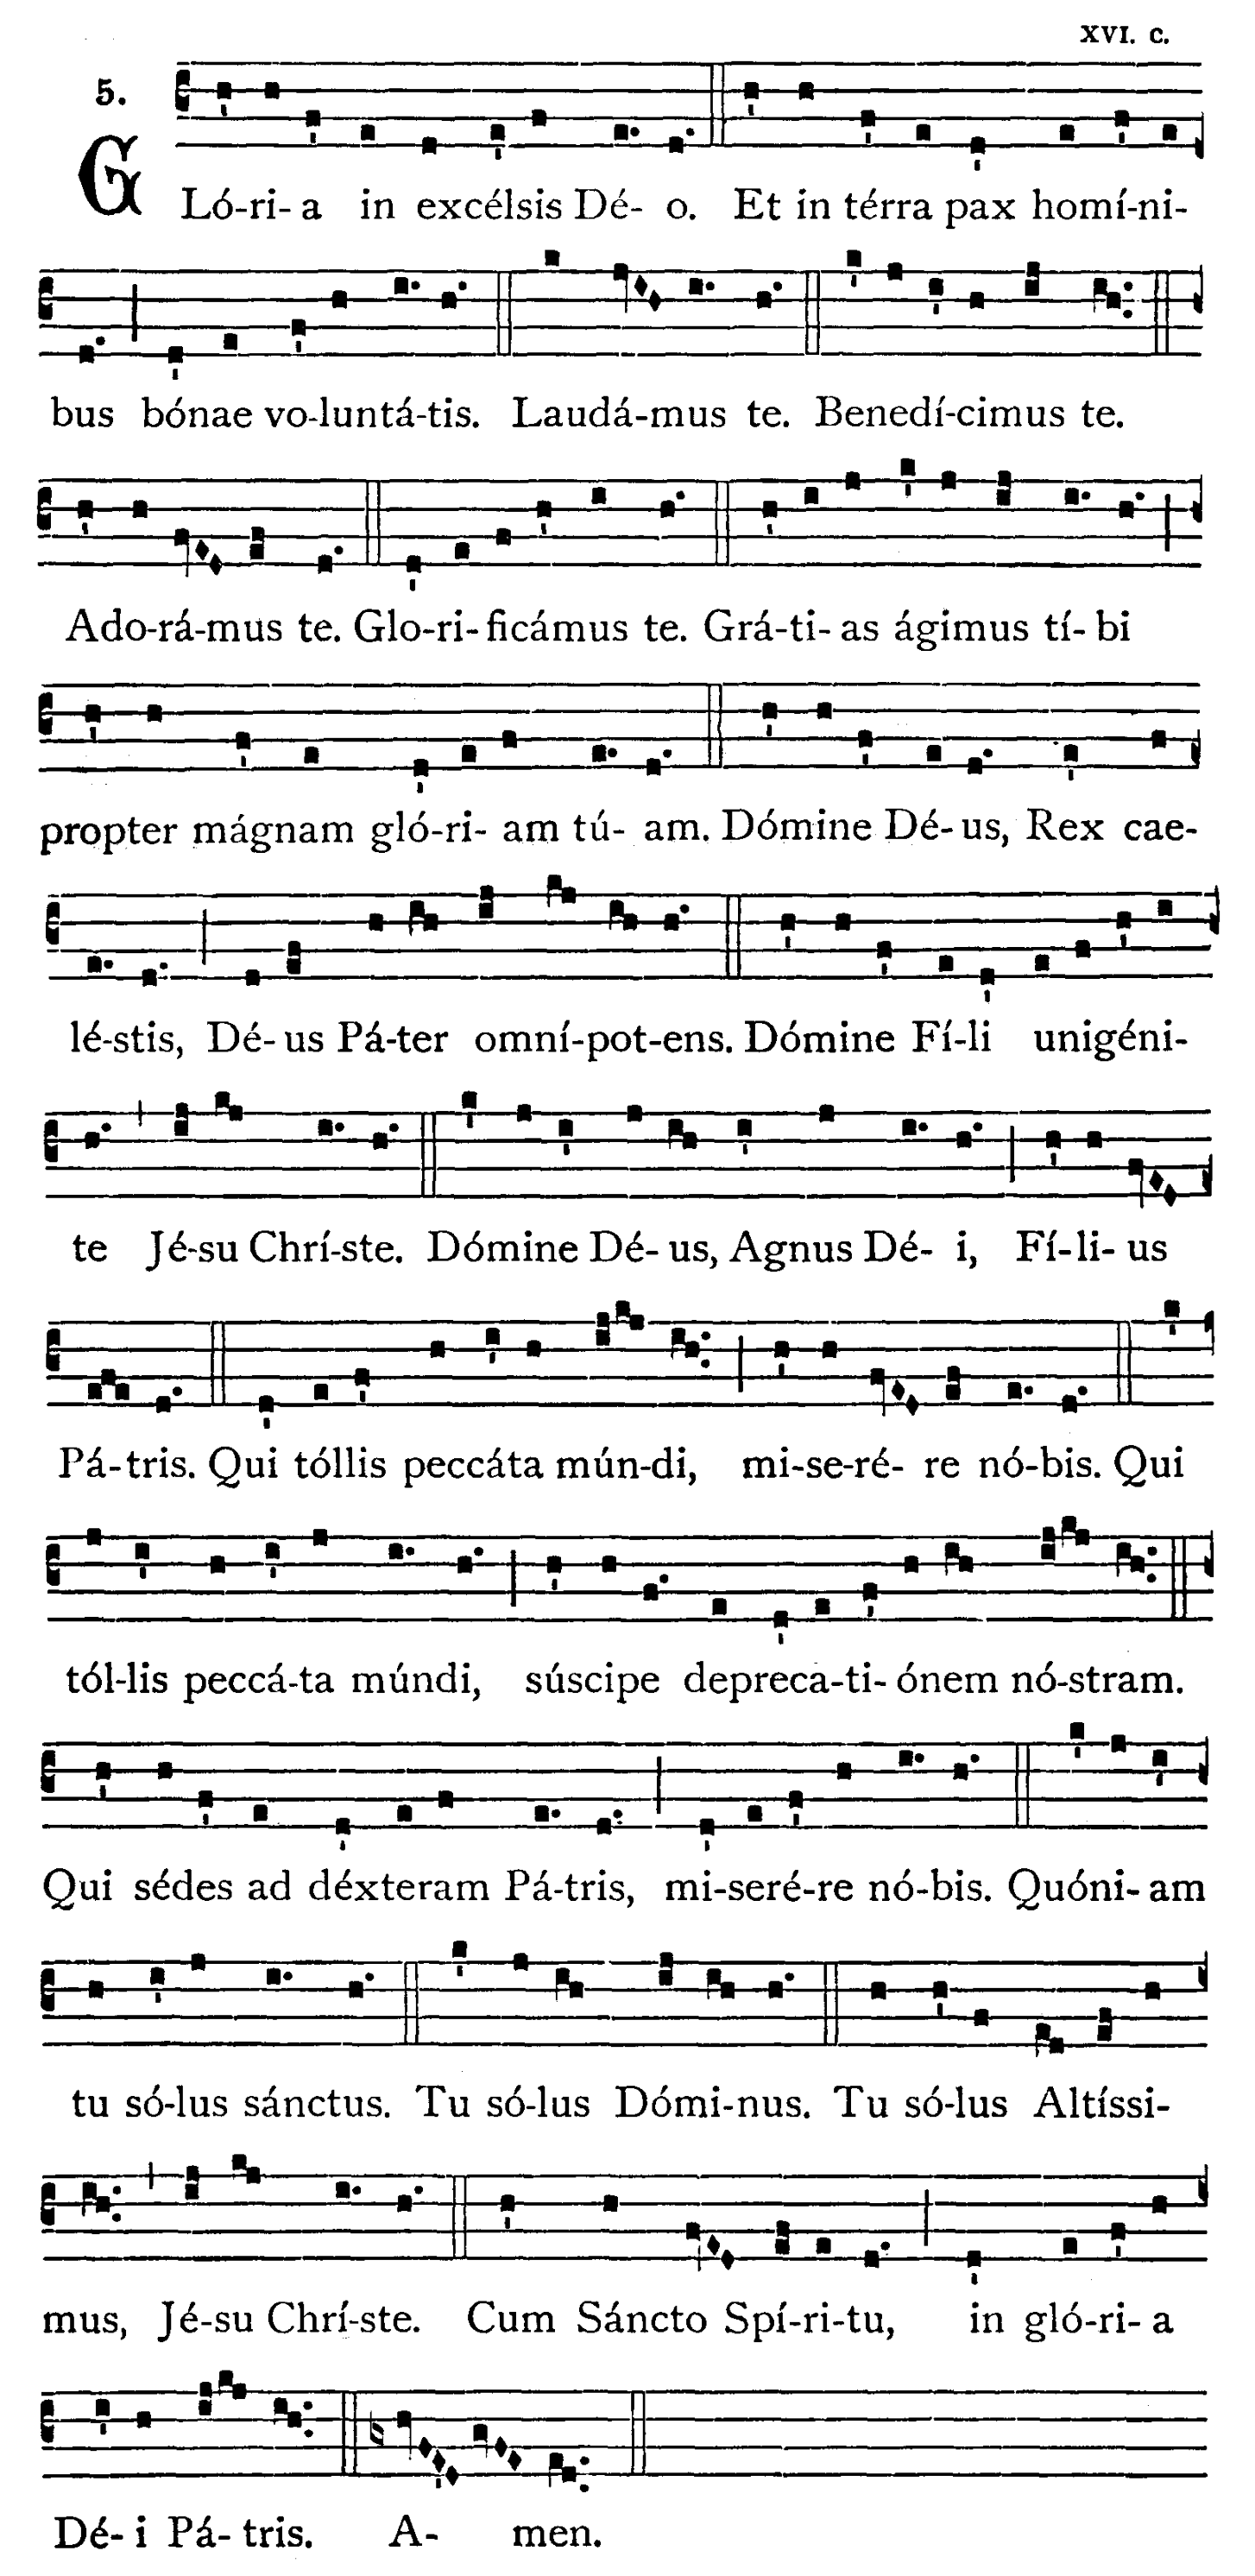
\includegraphics
        [scale=0.3, clip, viewport=1cm 53cm 50cm 105cm]
        {img/gloria.png}
\end{figure}

\begin{figure}[ht]
    \vspace*{2\baselineskip}
    \centering
    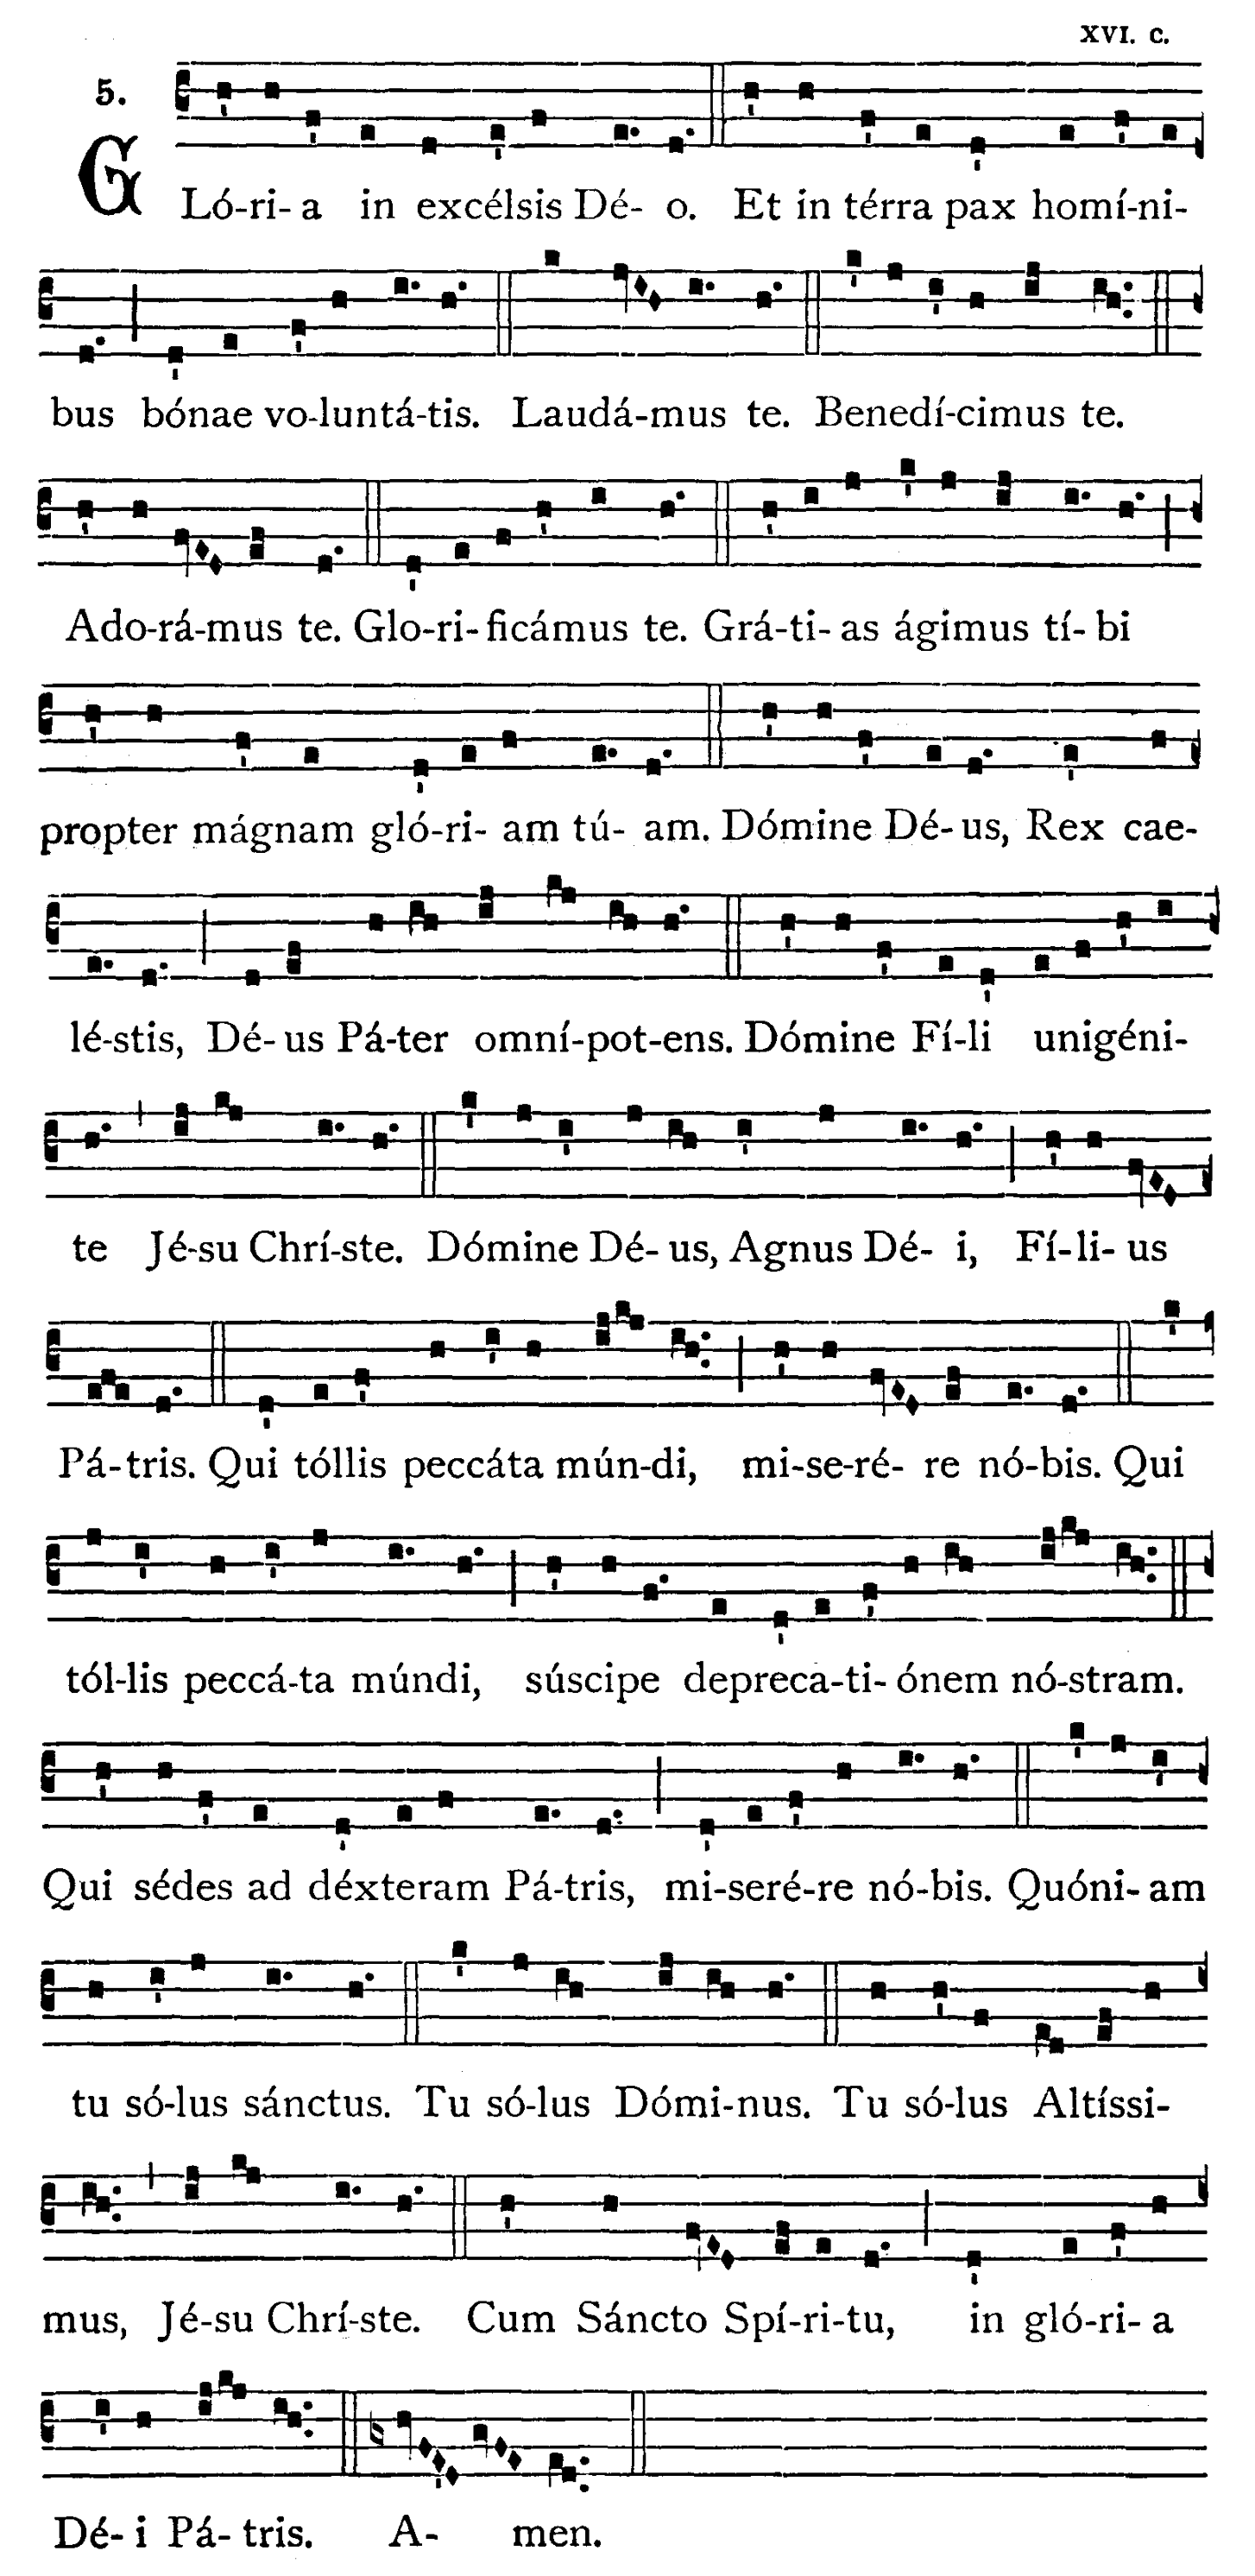
\includegraphics
        [scale=0.3, clip, viewport=1cm 1cm 50cm 53cm]
        {img/gloria.png}
    \vspace*{2\baselineskip}
\end{figure}

\textit{Postea in medio altaris extendens et iungens manus, caputque
aliquantulum inclinans, dicit, si dicendum est}, Gloria in excelsis Deo,
\textit{et prosequitur iunctis manibus.  Cum dicit} Adoramus te, Gratias agimus
tibi, \textit{et} Iesu Christe, et Suscipe deprecationem, \textit{inclinat
caput: et in fine dicens:} Cum Sancto Spiritu, \textit{signat se a fronte ad
pectus.}

\biblia{Lc. 2, 14}

\initialis{G}loria in excelsis Deo.  Et in terra pax hominibus bonae voluntatis.
Laudamus te.  Benedicimus te.  \directio{flectens} Adoramus te.  Glorificamus
te.  \directio{flectens} Gratias agimus tibi propter magnam gloriam tuam.
Domine Deus, Rex caelestis, Deus Pater omnipotens.  Domine Fili unigenite,
\directio{flectens} Iesu Christe.  Domine Deus, Agnus Dei, Filius Patris.  Qui
tollis peccata mundi, miserere nobis.  Qui tollis peccata mundi,
\directio{flectens} suscipe deprecationem nostram.  Qui sedes ad dexteram
Patris, miserere nobis.  Quoniam tu solus Sanctus.  Tu solus Dominus.  Tu solus
Altissimus, \directio{flectens} Iesu Christe.  \cross{} Cum Sancto Spiritu, in
gloria Dei Patris.  Amen.

\textit{Deinde osculatur altare in medio, et versus ad populum dicit:}

\versiculum{Dominus vobiscum.}
\alternatim{\par\responsorium{Et cum spiritu tuo.}}

\textit{Postea dicit:}

\versiculum{Oremus.}

\textit{%
    et orationes, unam aut plures, ut Ordo Officii postulat.  Sequitur Epistola,
    graduale, tractus, vel Alleluia cum versu, aut sequentia, prout Tempus aut
    qualitas Missae postulat.
}

\section{Collecta}

\proprius{Collecta}

\section{Epistola}

\directio{sedens}

\directio{proprius: Epistola}

\section{Graduale, Tractus, Alleluia, Sequentia}

\proprius{Graduale/Tractus/Alleluia/Sequentia}

\section{Evangelium}

\textit{%
    His finitis, si Missa est solemnis, diaconus librum Evangeliorum deponit
    super medium altaris, et, nisi sit Missa defunctorum, celebrans benedicit
    incensum, ut supra: deinde diaconus, genuflexus ante altare, manibus
    iunctis, dicit:
}

\initialis{M}unda cor meum ac labia mea, omnipotens Deus, qui labia Isaiae
prophetae calculo mundasti ignito: ita me tua grata miseratione dignare mundare,
ut sanctum Evangelium tuum digne valeam nuntiare.  Per Christum Dominum nostrum.
Amen.

\textit{%
    Postea accipit librum de altari, et rursus genuflexus petit benedictionem a
    sacerdote, dicens:
}

\versiculum{Iube, domne, benedicere.}

\textit{Sacerdos respondet:}

\initialis{D}ominus sit in corde tuo et in labiis tuis: ut digne et competenter
annunties Evangelium suum: In nomine Patris, Filii, \cross{} et Spiritus Sancti.
Amen.

\directio{stans}

\textit{%
    Et, accepta benedictione, osculatur manum celebrantis: et cum aliis
    ministris, incenso, et luminaribus, accedens ad locum Evangelii, stans
    iunctis manibus, dicit:
}

\versiculum{Dominus vobiscum.}
\alternatim{\par\responsorium{Et cum spiritu tuo.}}

\textit{Et pronuntians:}

\versiculum{Sequentia sancti Evangelii secundum N.}

\textit{sive} Initium, \textit{pollice dexterae manus signat librum in principio
Evangelii, quod est lecturus, deinde seipsum in fronte, ore, et pectore: et dum
ministri respondent:}

\directio{signans se in fronte, ore, et pectore}

\responsorium{Gloria tibi, Domine.}

\textit{incensat ter librum, postea prosequitur Evangelium iunctis manibus.}

\proprius{Evangelium}

\textit{%
    Quo finito, subdiaconus defert librum sacerdoti, qui osculatur Evangelium,
    dicens:
}

\sacerdos{Per evangelica dicta deleantur nostra delicta.}

\textit{Deinde sacerdos incensatur a diacono.}

\divisio

\textit{Si vero sacerdos sine diacono et subdiacono celebrat, delato libro ad
aliud latus altaris, inclinatus in medio, iunctis manibus dicit} Munda cor meum,
\textit{ut supra, et} Iube, Domine, benedicere.  Dominus sit in corde meo
et in labiis meis: ut digne et competenter annuntiem Evangelium suum.  Amen.

\textit{Deinde, conversus ad librum, iunctis manibus, dicit}:

\versiculum{Dominus vobiscum.}
\alternatim{\par\responsorium{Et cum spiritu tuo.}}

\textit{Et pronuntians}:

\versiculum{Initium (\textit{sive} Sequentia) sancti Evangelii.}

\textit{%
    signat librum, et se in fronte, ore, et pectore, et legit Evangelium, ut
    dictum est.  Quo finito, respondet minister:
}

\responsorium{Laus tibi, Christe.}

\textit{et sacerdos osculatur Evangelium, dicens:}

\sacerdos{Per evangelica dicta\ldots (\textit{ut supra})}

\textit{In Missis defunctorum dicitur} Munda cor meum, \textit{sed non petitur
benedictio, non deferuntur luminaria, nec celebrans osculatur librum.}

\divisio

\section{Credo}

\begin{wrapfigure}{r}{0.5\textwidth}
    \centering
    \vspace{-0.5\baselineskip}
    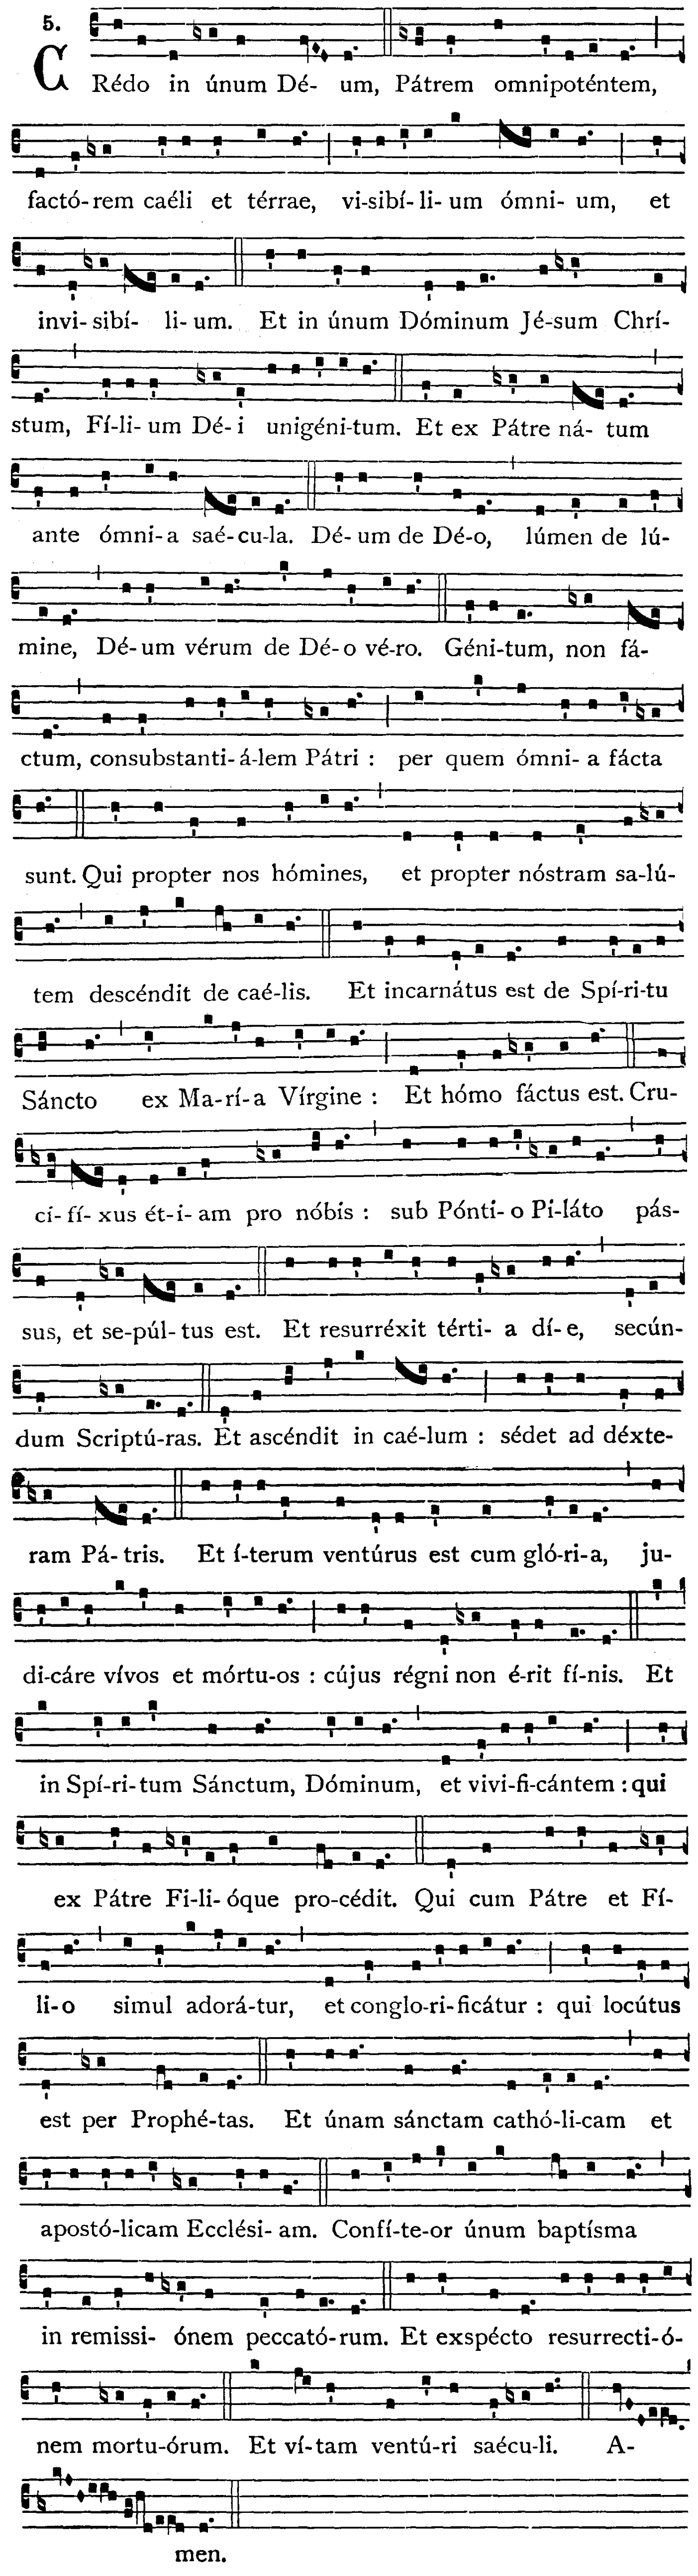
\includegraphics
        [scale=0.3, clip, viewport=2cm 175.5cm 27.25cm 183cm]
        {img/credo.png}
    \vspace{-0.5\baselineskip}
\end{wrapfigure}

\textit{Deinde ad medium altaris extendens, elevans et iungens manus, dicit, si
dicendum est}, Credo in unum Deum, \textit{et prosequitur iunctis manibus.  Cum
dicit} Deum, \textit{caput cruci inclinat: quod similiter facit, cum dicit}
Iesum Christum, \textit{et} simul adoratur.  \textit{Ad illa autem verba} Et
incarnatus est, \textit{genuflectit usque dum dicatur} Et homo factus est.
\textit{In fine ad} Et vitam venturi saeculi, \textit{signat se signo crucis a
fronte ad pectus.}

\initialis{C}redo in unum Deum, Patrem omnipotentem, factorem caeli et terrae,
visibilium omnium et invisibilium.  Et in unum Dominum \directio{flectens} Iesum
Christum, Filium Dei unigenitum.  Et ex Patre natum ante omnia saecula.  Deum de
Deo, lumen de lumine, Deum verum de Deo vero.  Genitum, non factum,
consubstantialem Patri: per quem omnia facta sunt.  Qui propter nos homines et
propter nostram salutem descendit de caelis.  \directio{genuflectens} \textsc{Et
incarnatus est de Spiritu Sancto ex Maria Virgine: et homo factus est}.
Crucifixus etiam pro nobis: sub Pontio Pilato passus, et sepultus est.  Et
resurrexit tertia die, secundum Scripturas.  Et ascendit in caelum: sedet ad
dexteram Patris.  Et iterum venturus est cum gloria iudicare vivos et mortuus:
cuius regni non erit finis.  Et in Spiritum Sanctum, Dominum, et vivificantem:
qui ex Patre Filioque procedit.  Qui cum Patre et Filio \directio{flectens}
simul adoratur et conglorificatur: qui locutus est per Prophetas.  Et unam
sanctam catholicam et apostolicam Ecclesiam.  Confiteor unum baptisma in
remissionem peccatorum.  Et exspecto resurrectionem mortuorum.  \cross{} Et
vitam venturi saeculi.  Amen.

\begin{center}
    \vspace*{\fill}
    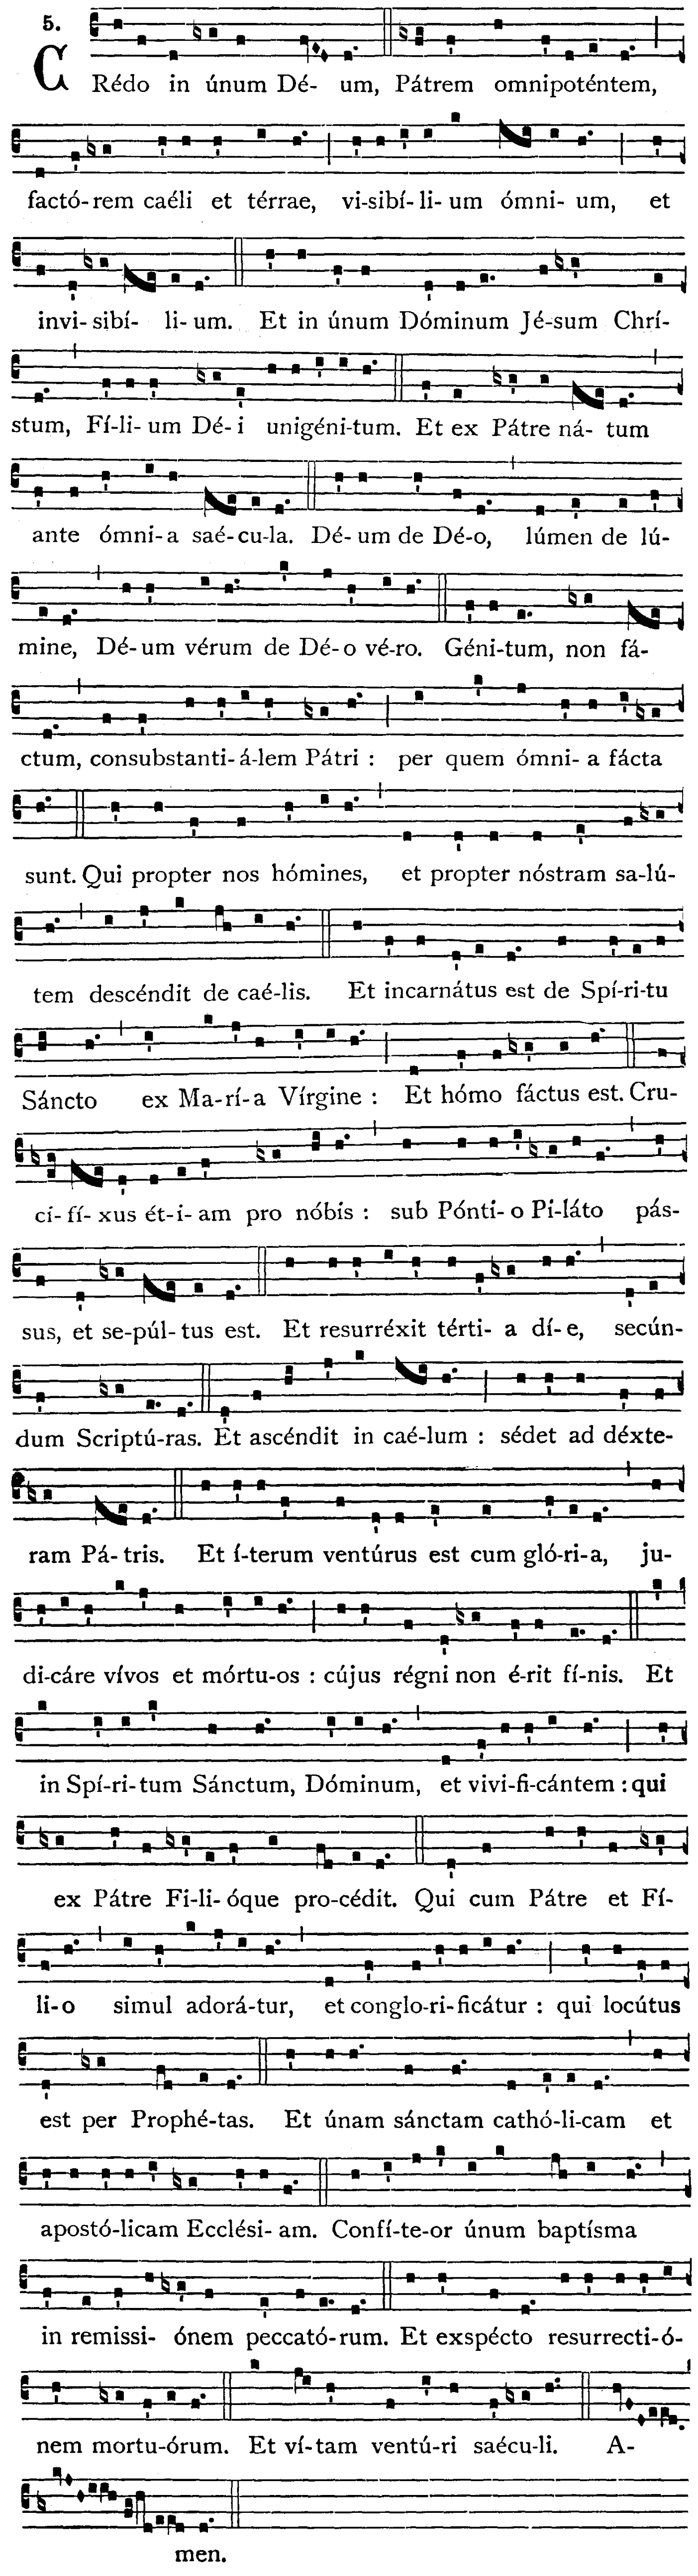
\includegraphics
        [scale=0.3, clip, viewport=0cm 159cm 49.25cm 183cm]
        {img/credo.png}
    \vspace*{\fill}
    \pagebreak
    \vspace*{\fill}
    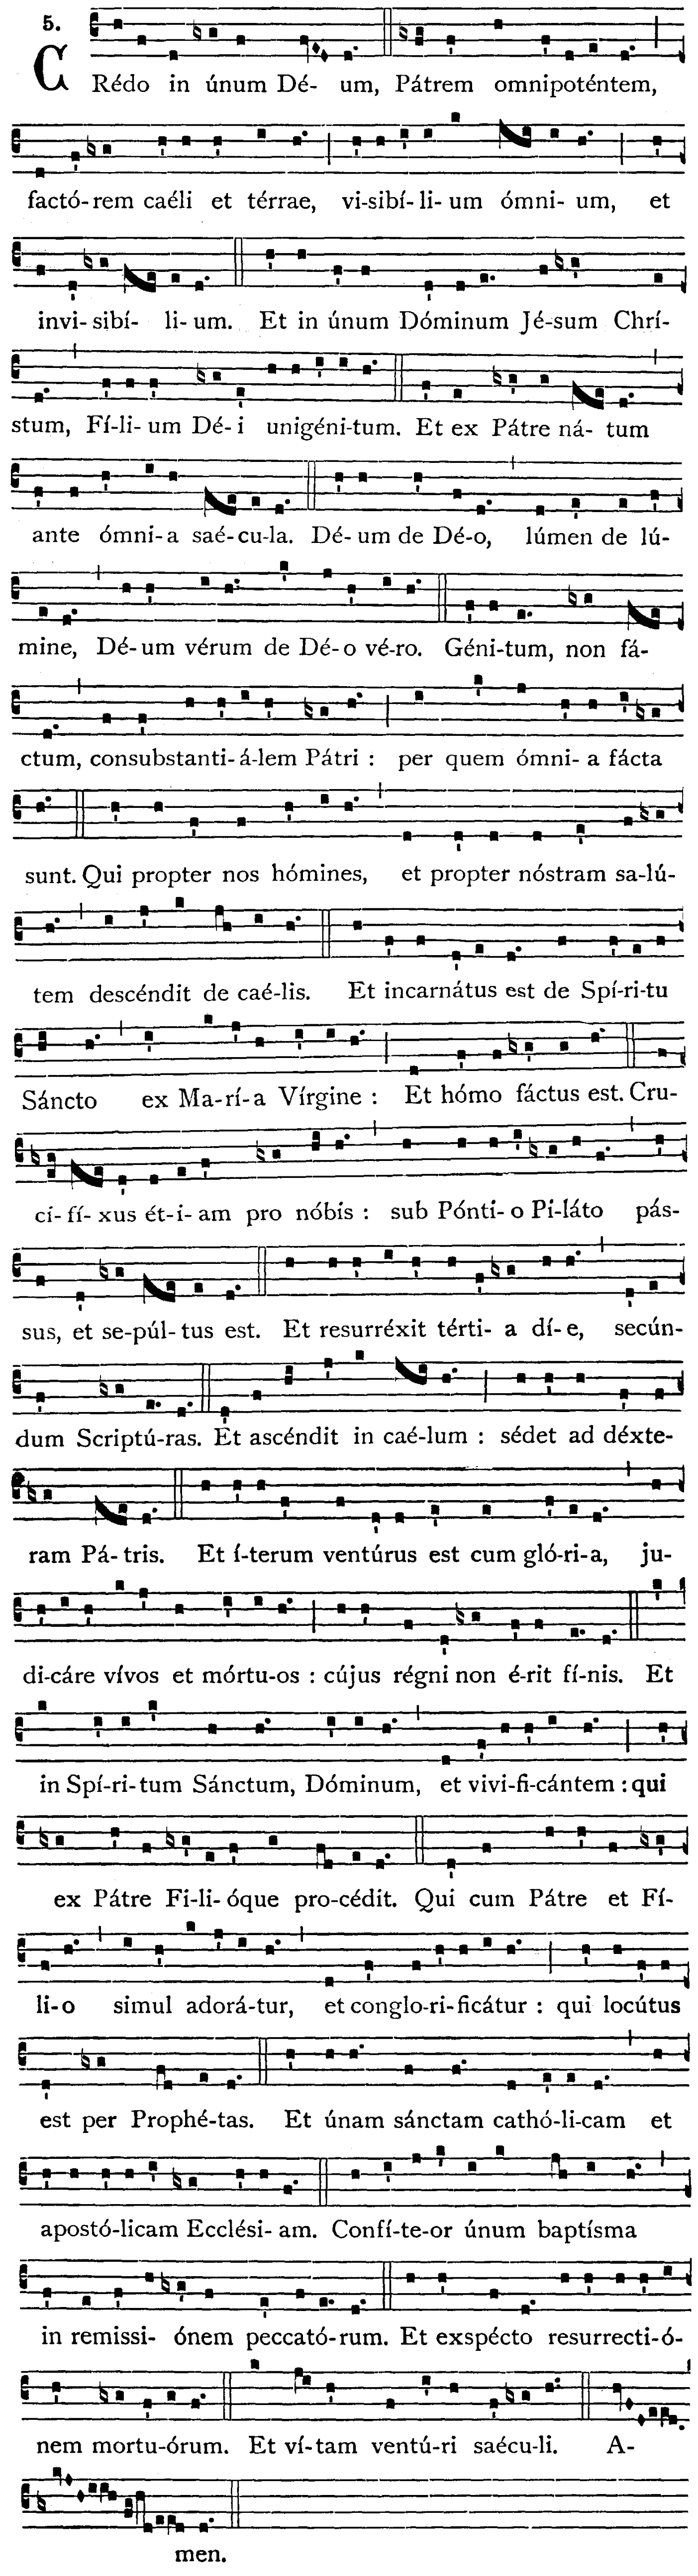
\includegraphics
        [scale=0.3, clip, viewport=0cm 80cm 49.25cm 158cm]
        {img/credo.png}
    \vspace*{\fill}
    \pagebreak
    \vspace*{\fill}
    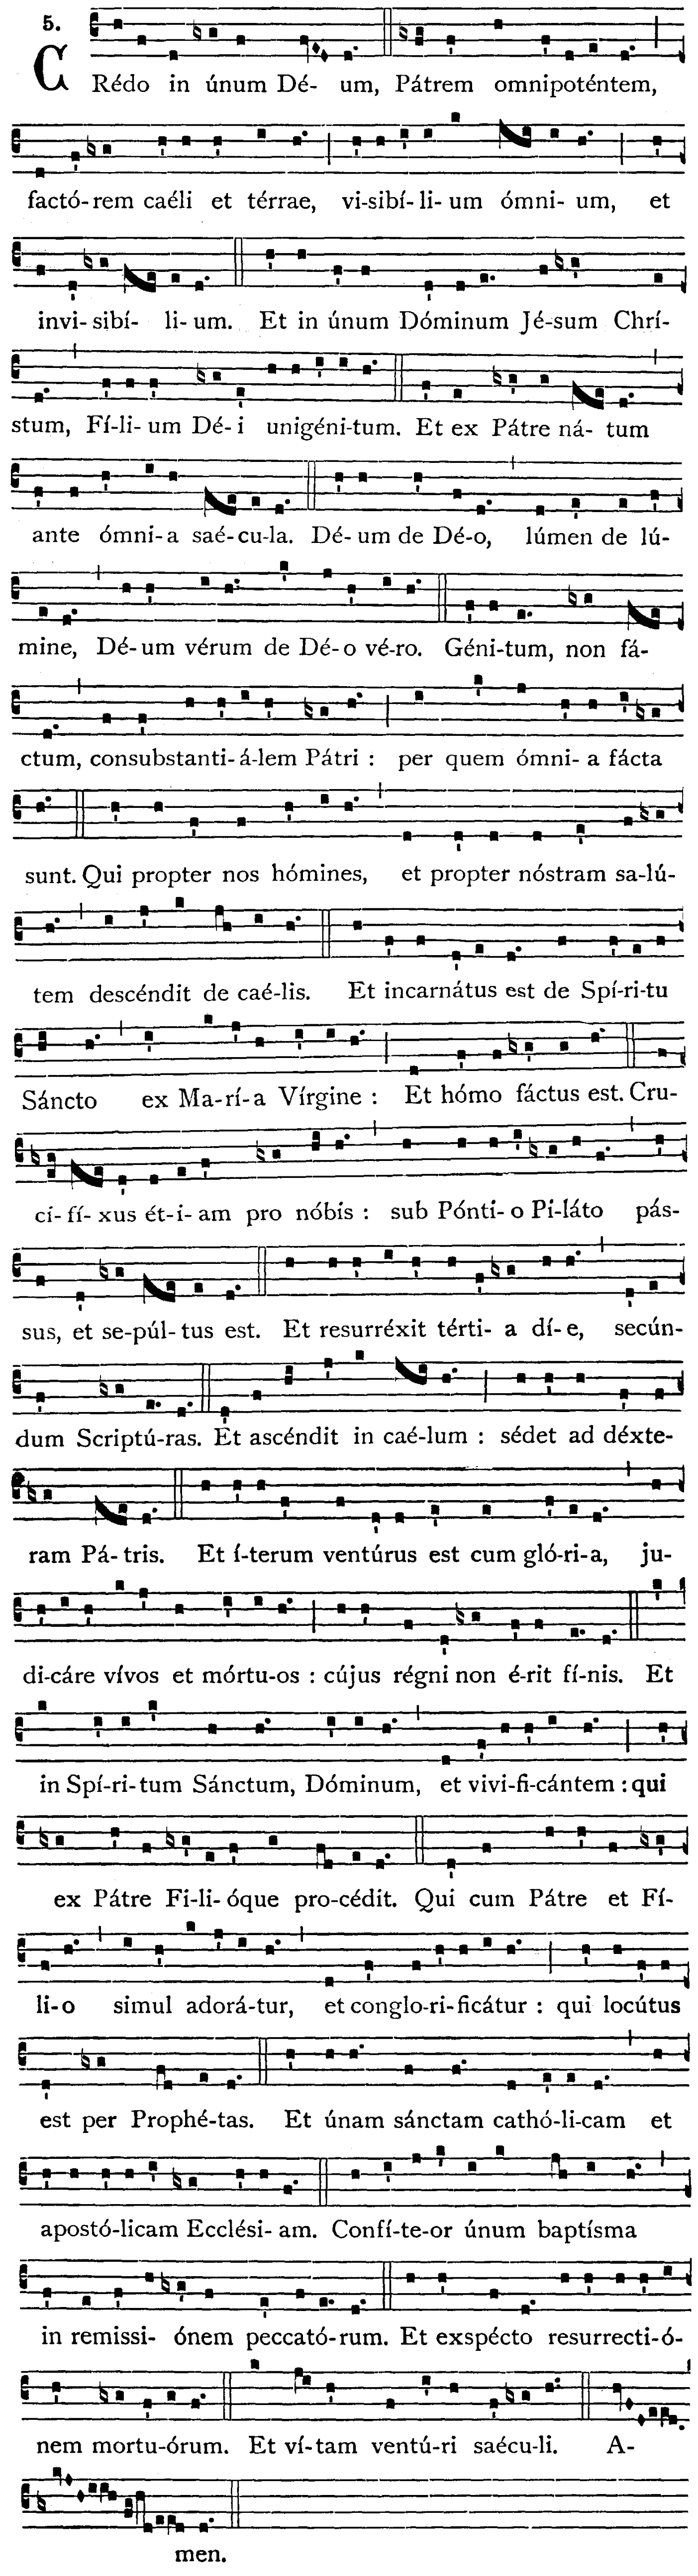
\includegraphics
        [scale=0.3, clip, viewport=0cm 0cm 49.25cm 79cm]
        {img/credo.png}
    \vspace*{\fill}
\end{center}
